\documentclass[12pt]{article}
\usepackage{float}
\usepackage{graphicx}
\usepackage{svg}
\title{Key West Annual Temperatures}
\author{Abigail Rossina Millward}
\date{1st of November 2017}
\begin{document}
	\maketitle
	Is the temperature of one year significantly correlated with the next year (successive years), across the years?
	
	\begin{abstract}
		The aim of this assignment was to see if the temperatures collected
		at Key West in Florida were significantly correlated with the next year.
	\end{abstract}
	
	\section{Results}
		
	\begin{figure}[H]
			\centering
	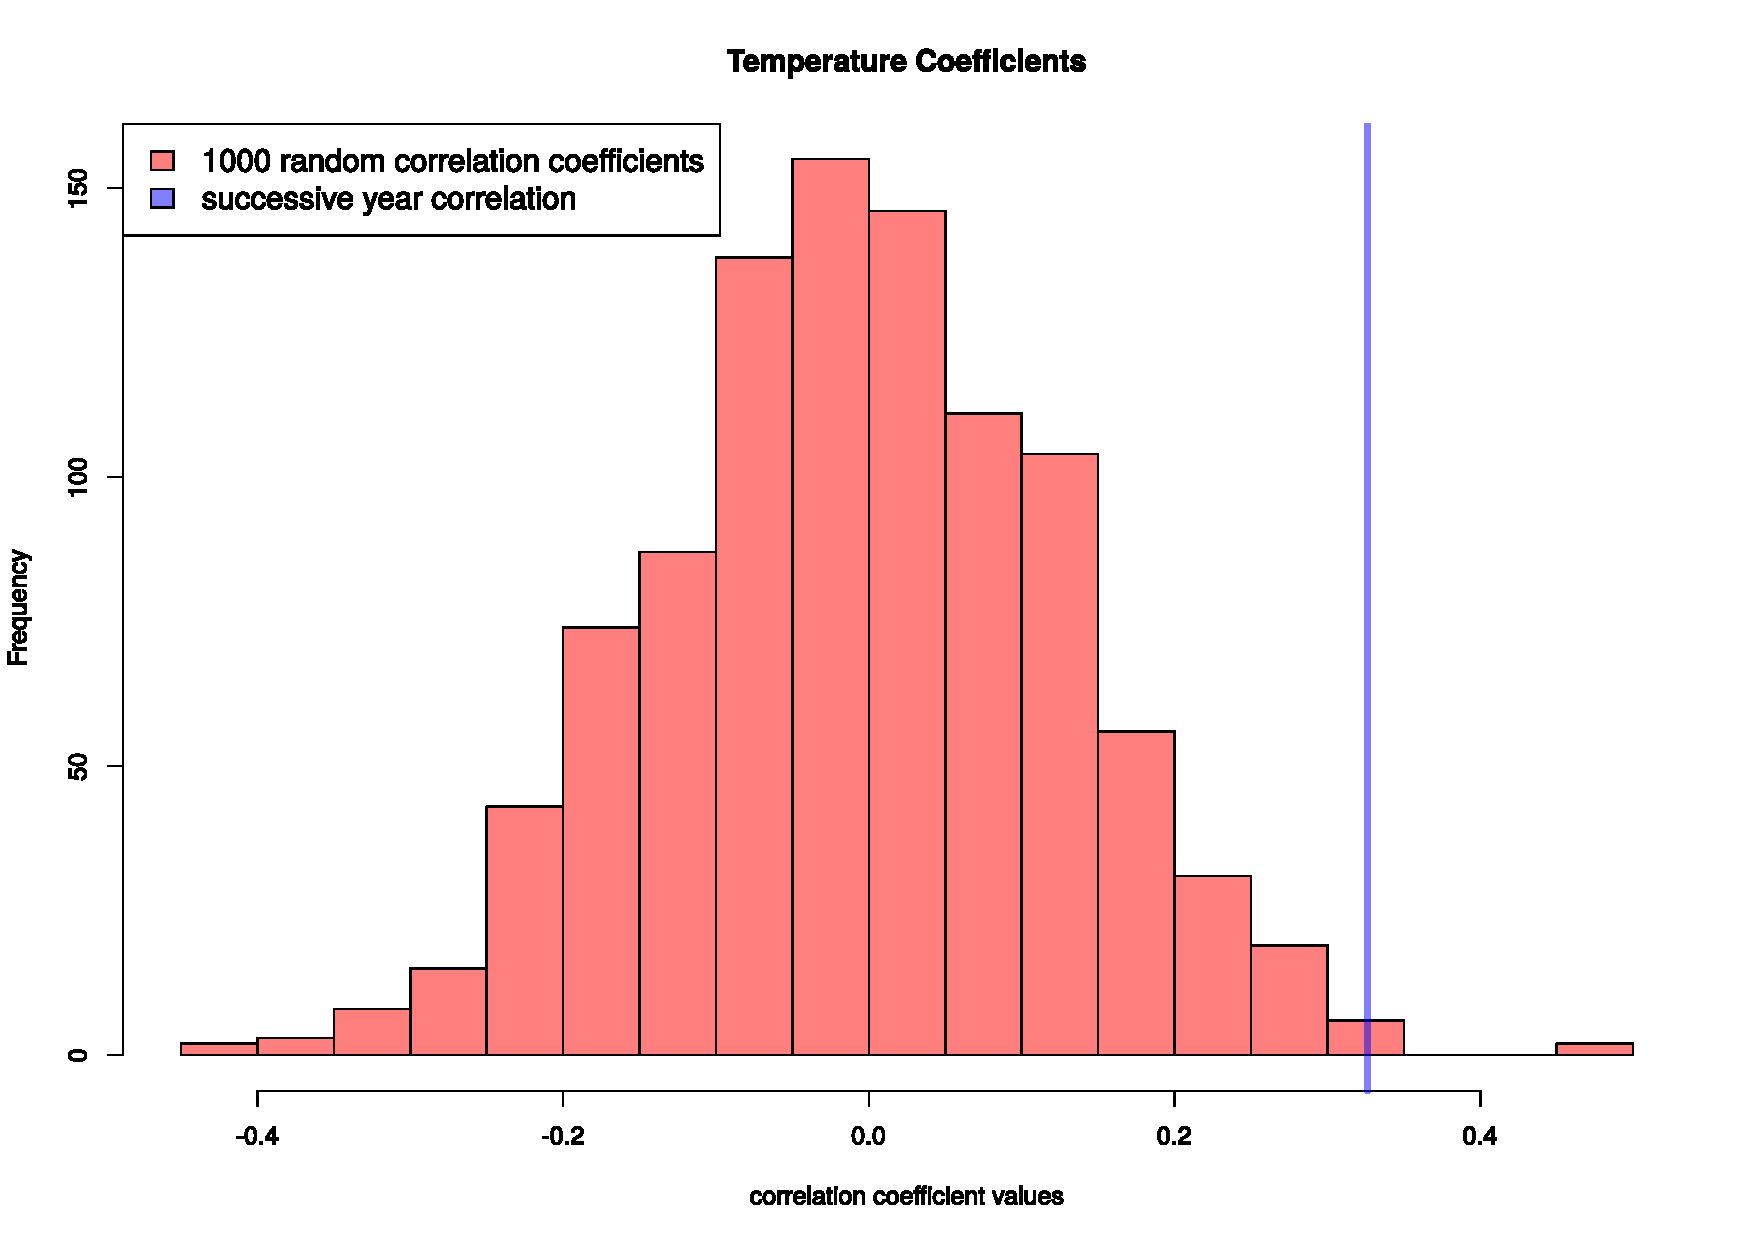
\includegraphics[scale=.4]{TAutoCorr1.pdf}
			\caption{Temperature in Key West, Florida from 1901-2000.}
	\label{fig:TAutoCorrsvg1}
	\end{figure}

	\section{Interpretation}
	Figure 1 shows a graph with a significantly positive correlation between t and t-1 years. The positive correlation shown in the graph is further backed up by a pearsons correlation value of 0.33, which was attained by computing t$(x_time)$ and t-1$(y_time)$ years using the $cor()$ function in R, and a p value of $~ 0.003$ indicating these results are extremely unlikely to arise by chance. Hence, it can be interpreted that one years temperature is indicative of the subsequent years temperature.
	
	\end{document}
